\apendice{Especificación de Requisitos}


Este apéndice recoge la especificación funcional del sistema desarrollado, incluyendo los casos de uso definidos, los requisitos asociados y los prototipos de interacción implementados en la aplicación. Su objetivo es proporcionar una visión estructurada de las funcionalidades del sistema desde la perspectiva del usuario final.

Los principales casos de uso definidos son:

\begin{itemize}
  \item CU-1 – Introducir datos clínicos
  \item CU-2 – Ejecutar predicción
  \item CU-3 – Interpretar resultado con SHAP
  \item CU-4 – Generar informe PDF
\end{itemize}

\section{Diagrama de casos de uso}

El diagrama que se muestra a continuación representa gráficamente los principales casos de uso del sistema desde la perspectiva del usuario. Cada uno de estos casos está descrito en detalle en las secciones posteriores de este apéndice.

\begin{figure}[H]
    \centering
    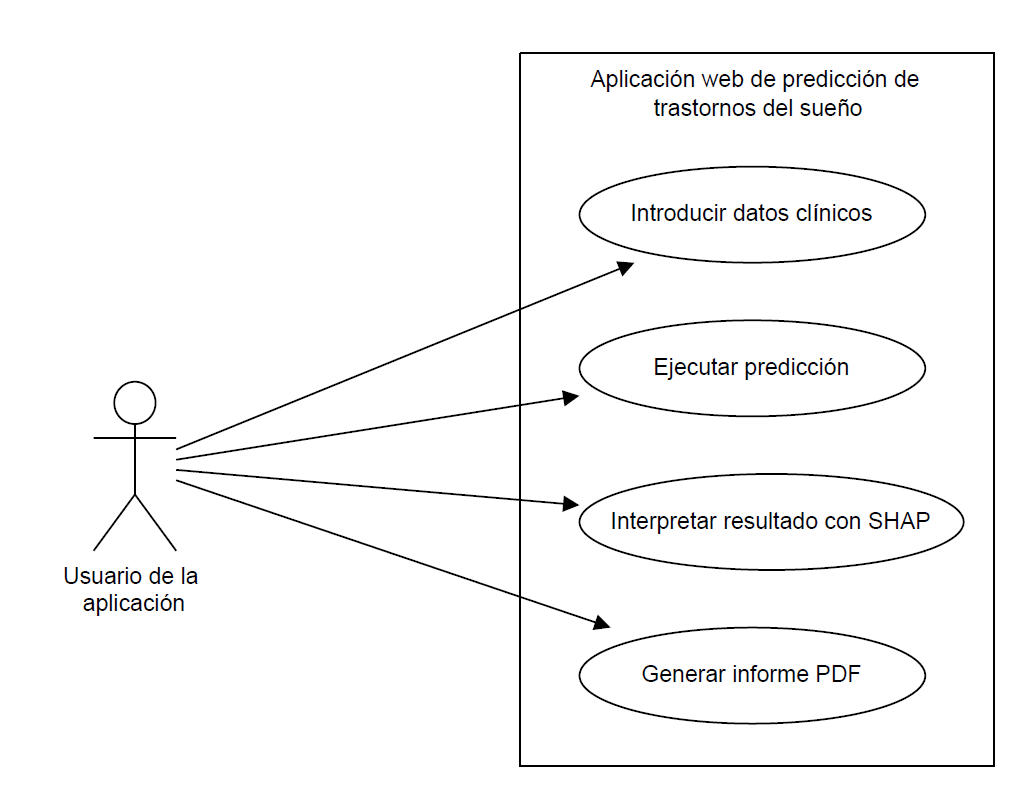
\includegraphics[width=0.9\linewidth]{img/diagrama_casos_uso.png}
    \caption{Diagrama de casos de uso de la aplicación web.}
    \label{fig:casos-uso}
\end{figure}

\section{Explicación casos de uso}

\subsection{CU-1 – Introducir datos clínicos}

\begin{table}[!htbp]
	\centering
	\begin{tabularx}{\linewidth}{ p{0.21\columnwidth} p{0.71\columnwidth} }
		\toprule
		\textbf{CU-1}    & Introducir datos clínicos \\
		\toprule
		\textbf{Versión}              & 1.0    \\
		\textbf{Autor}                & Marina Martín Marijuán \\
		\textbf{Requisitos asociados} & RF-01, RF-02 \\
		\textbf{Descripción}          & El usuario introduce las variables clínicas y de estilo de vida necesarias para realizar la predicción. \\
		\textbf{Precondición}         & La aplicación ha sido cargada correctamente en el navegador. \\
		\textbf{Acciones}             &
		\begin{enumerate}
			\item Acceder al formulario.
			\item Introducir edad, género, ocupación, duración/calidad del sueño, IMC, estrés, FC, PA, pasos.
			\item Revisar y validar que los datos introducidos cumplen el formato requerido.
		\end{enumerate}\\
		\textbf{Postcondición}        & El sistema almacena los datos temporalmente y permite realizar la predicción. \\
		\textbf{Excepciones}          & Algún campo no válido o sin completar. El sistema muestra advertencia. \\
		\textbf{Importancia}          & Alta \\
		\bottomrule
	\end{tabularx}
	\caption{CU-1 Introducir datos clínicos.}
\end{table}

\begin{samepage}
\subsection{CU-2 – Ejecutar predicción}

\begin{table}[!htbp]
	\centering
	\begin{tabularx}{\linewidth}{ p{0.21\columnwidth} p{0.71\columnwidth} }
		\toprule
		\textbf{CU-2}    & Ejecutar predicción \\
		\toprule
		\textbf{Versión}              & 1.0    \\
		\textbf{Autor}                & Marina Martín Marijuán \\
		\textbf{Requisitos asociados} & RF-03 \\
		\textbf{Descripción}          & El sistema ejecuta la predicción del trastorno del sueño en función de los datos introducidos. \\
		\textbf{Precondición}         & Formulario completo con datos válidos. \\
		\textbf{Acciones}             &
		\begin{enumerate}
			\item Pulsar botón “Realizar predicción”.
			\item Ejecutar modelo y obtener clase predicha con probabilidades.
		\end{enumerate}\\
		\textbf{Postcondición}        & Se muestra el resultado de la predicción en pantalla. \\
		\textbf{Excepciones}          & Error de ejecución del modelo o fallo en la interfaz. \\
		\textbf{Importancia}          & Alta \\
		\bottomrule
	\end{tabularx}
	\caption{CU-2 Ejecutar predicción.}
\end{table}
\end{samepage}

\subsection{CU-3 – Interpretar resultado}

\begin{table}[!htbp]
	\centering
	\begin{tabularx}{\linewidth}{ p{0.21\columnwidth} p{0.71\columnwidth} }
		\toprule
		\textbf{CU-3}    & Interpretar resultado con SHAP \\
		\toprule
		\textbf{Versión}              & 1.0    \\
		\textbf{Autor}                & Marina Martín Marijuán \\
		\textbf{Requisitos asociados} & RF-04 \\
		\textbf{Descripción}          & Se muestran dos gráficos SHAP: uno individual que explica la predicción concreta realizada para el usuario, y otro global que representa la importancia de cada variable en el modelo. \\
		\textbf{Precondición}         & Se ha realizado una predicción. \\
		\textbf{Acciones}             &
		\begin{enumerate}
			\item Visualizar los gráficos SHAP generado.
			\item Analizar variables con mayor peso positivo o negativo en ambos contextos.
		\end{enumerate}\\
		\textbf{Postcondición}        & El usuario comprende los factores que han influido en su predicción individual, así como los que el modelo considera más relevantes de forma general. \\
		\textbf{Excepciones}          & Alguno de los gráficos no se carga correctamente. \\
		\textbf{Importancia}          & Media \\
		\bottomrule
	\end{tabularx}
	\caption{CU-3 Interpretar resultado con SHAP.}
\end{table}


\subsection{CU-4 – Generar informe PDF}

\begin{table}[!htbp]
	\centering
	\begin{tabularx}{\linewidth}{ p{0.21\columnwidth} p{0.71\columnwidth} }
		\toprule
		\textbf{CU-4}    & Generar informe PDF \\
		\toprule
		\textbf{Versión}              & 1.0    \\
		\textbf{Autor}                & Marina Martín Marijuán \\
		\textbf{Requisitos asociados} & RF-05 \\
		\textbf{Descripción}          & El sistema permite descargar un informe en PDF con los datos introducidos, resultados y explicación visual. \\
		\textbf{Precondición}         & El sistema ya ha generado la predicción. \\
		\textbf{Acciones}             &
		\begin{enumerate}
			\item Pulsar botón “Descargar informe”.
			\item El sistema genera el archivo PDF.
		\end{enumerate}\\
		\textbf{Postcondición}        & El usuario dispone del archivo descargado localmente. \\
		\textbf{Excepciones}          & Error en la generación o guardado del informe. \\
		\textbf{Importancia}          & Alta \\
		\bottomrule
	\end{tabularx}
	\caption{CU-4 Generar informe PDF.}
\end{table}

\clearpage
\subsection{Resumen de requisitos funcionales y casos de uso asociados}

\begin{table}[H]
\centering
\begin{tabular}{|c|l|l|}
\hline
\textbf{Requisito} & \textbf{Descripción} & \textbf{Casos de uso asociados} \\
\hline
RF-01 & Introducción de datos personales & CU-1 \\
RF-02 & Validación de entrada & CU-1 \\
RF-03 & Ejecución del modelo & CU-2 \\
RF-04 & Visualización interpretativa (SHAP) & CU-3 \\
RF-05 & Generación del informe PDF & CU-4 \\
\hline
\end{tabular}
\caption{Relación entre requisitos funcionales y casos de uso.}
\label{tab:resumen-rf-cu}
\end{table}

\section{Prototipos de interfaz o interacción con el proyecto}

A continuación se presentan capturas reales de la aplicación web desarrollada, que ilustran las principales interacciones del usuario con el sistema. Estas imágenes complementan los casos de uso definidos previamente y muestran visualmente cómo se lleva a cabo cada acción funcional.

La Figura~\ref{fig:formulario-app} muestra el formulario principal en el que el usuario introduce sus datos clínicos y de estilo de vida. Este formulario recoge variables como edad, género, ocupación, duración y calidad del sueño, frecuencia cardíaca, presión arterial, nivel de estrés e índice de masa corporal, entre otras. El diseño del formulario ha sido concebido para ser accesible y usable tanto desde dispositivos de escritorio como móviles.

Una vez introducidos los datos, el usuario puede ejecutar la predicción y visualizar el resultado, como se aprecia en la Figura~\ref{fig:prediccion}. La aplicación muestra las probabilidades estimadas para cada clase (insomnio, apnea del sueño o ausencia de trastornos), de forma clara y visualmente destacada.

Además del resultado numérico, el sistema ofrece una interpretación visual del modelo mediante gráficos SHAP. En la Figura~\ref{fig:shap-global} se representa la importancia relativa de cada variable en la predicción a nivel global. La Figura~\ref{fig:shap-individual} muestra, por su parte, una explicación individualizada para un caso concreto, facilitando la comprensión personalizada del diagnóstico sugerido.

Finalmente, si el usuario lo desea, puede generar un informe en formato PDF con todos los datos introducidos, el resultado de la predicción y los gráficos de explicación, como se muestra en la Figura~\ref{fig:pdf-app}. El informe puede ser descargado localmente y está diseñado con un formato clínico que facilita su uso profesional.

Cada una de estas pantallas se corresponde con uno o varios de los casos de uso descritos en este anexo, y permite validar que la interfaz implementada satisface los requisitos funcionales definidos para el sistema.

\begin{figure}[H]
    \centering
    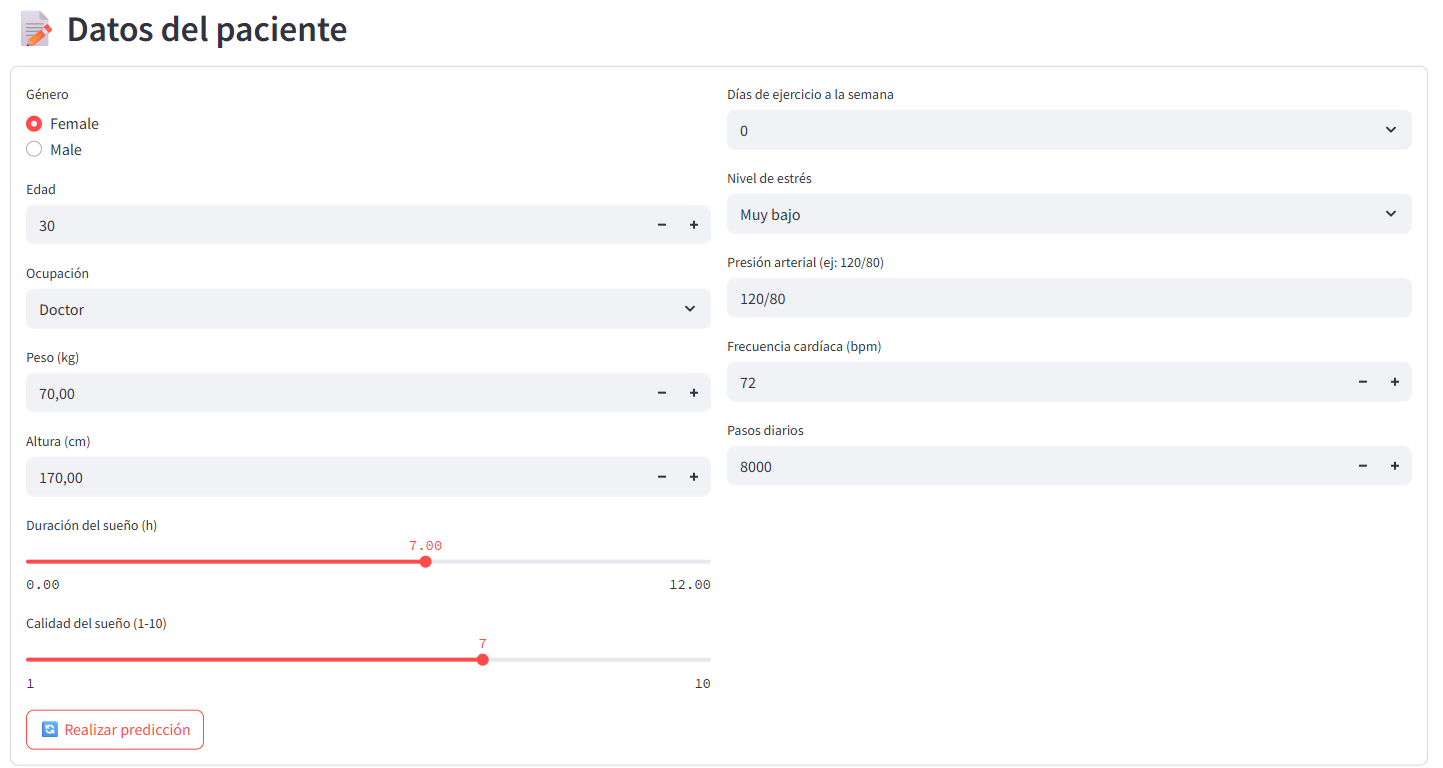
\includegraphics[width=0.9\linewidth]{img/formularioApp.png}
    \caption{Formulario de entrada de datos clínicos y de estilo de vida.}
    \label{fig:formulario-app}
\end{figure}

\begin{figure}[H]
    \centering
    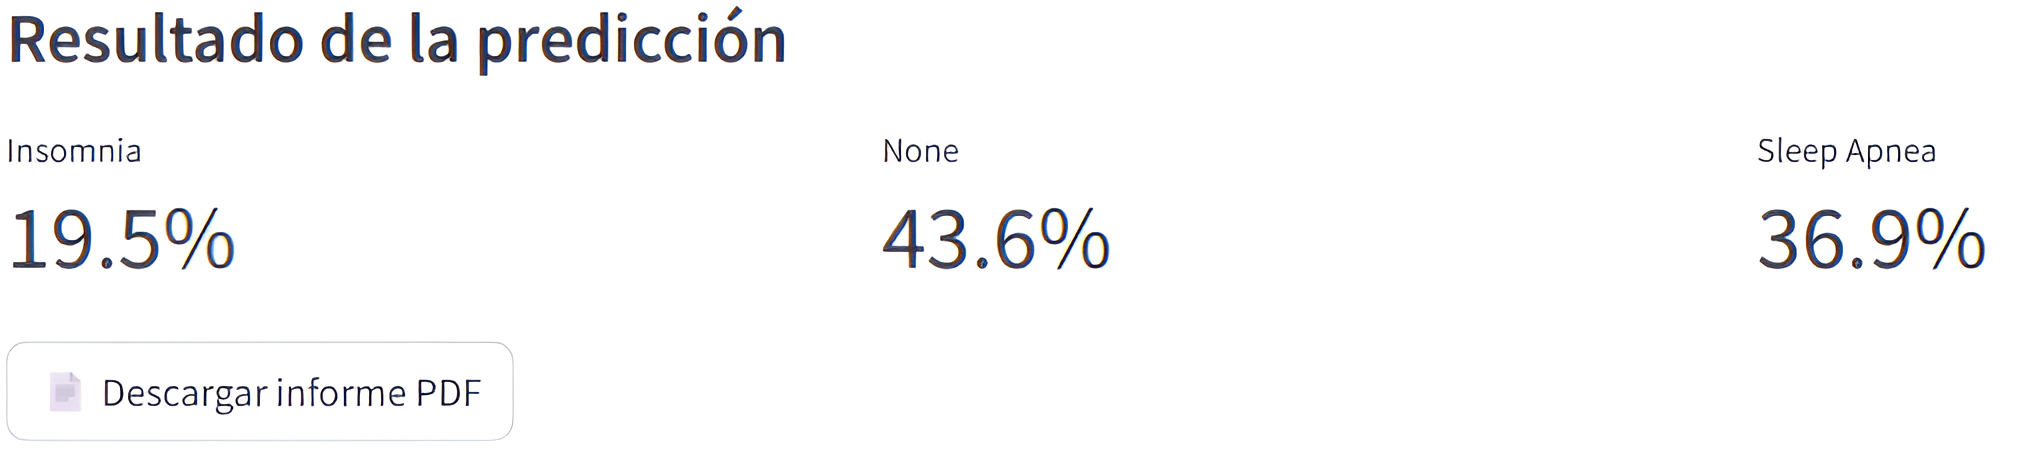
\includegraphics[width=0.9\linewidth]{img/resultadoPredd.png}
    \caption{Resultado de la predicción en pantalla, con distribución porcentual por clase.}
    \label{fig:prediccion}
\end{figure}

\begin{figure}[H]
    \centering
    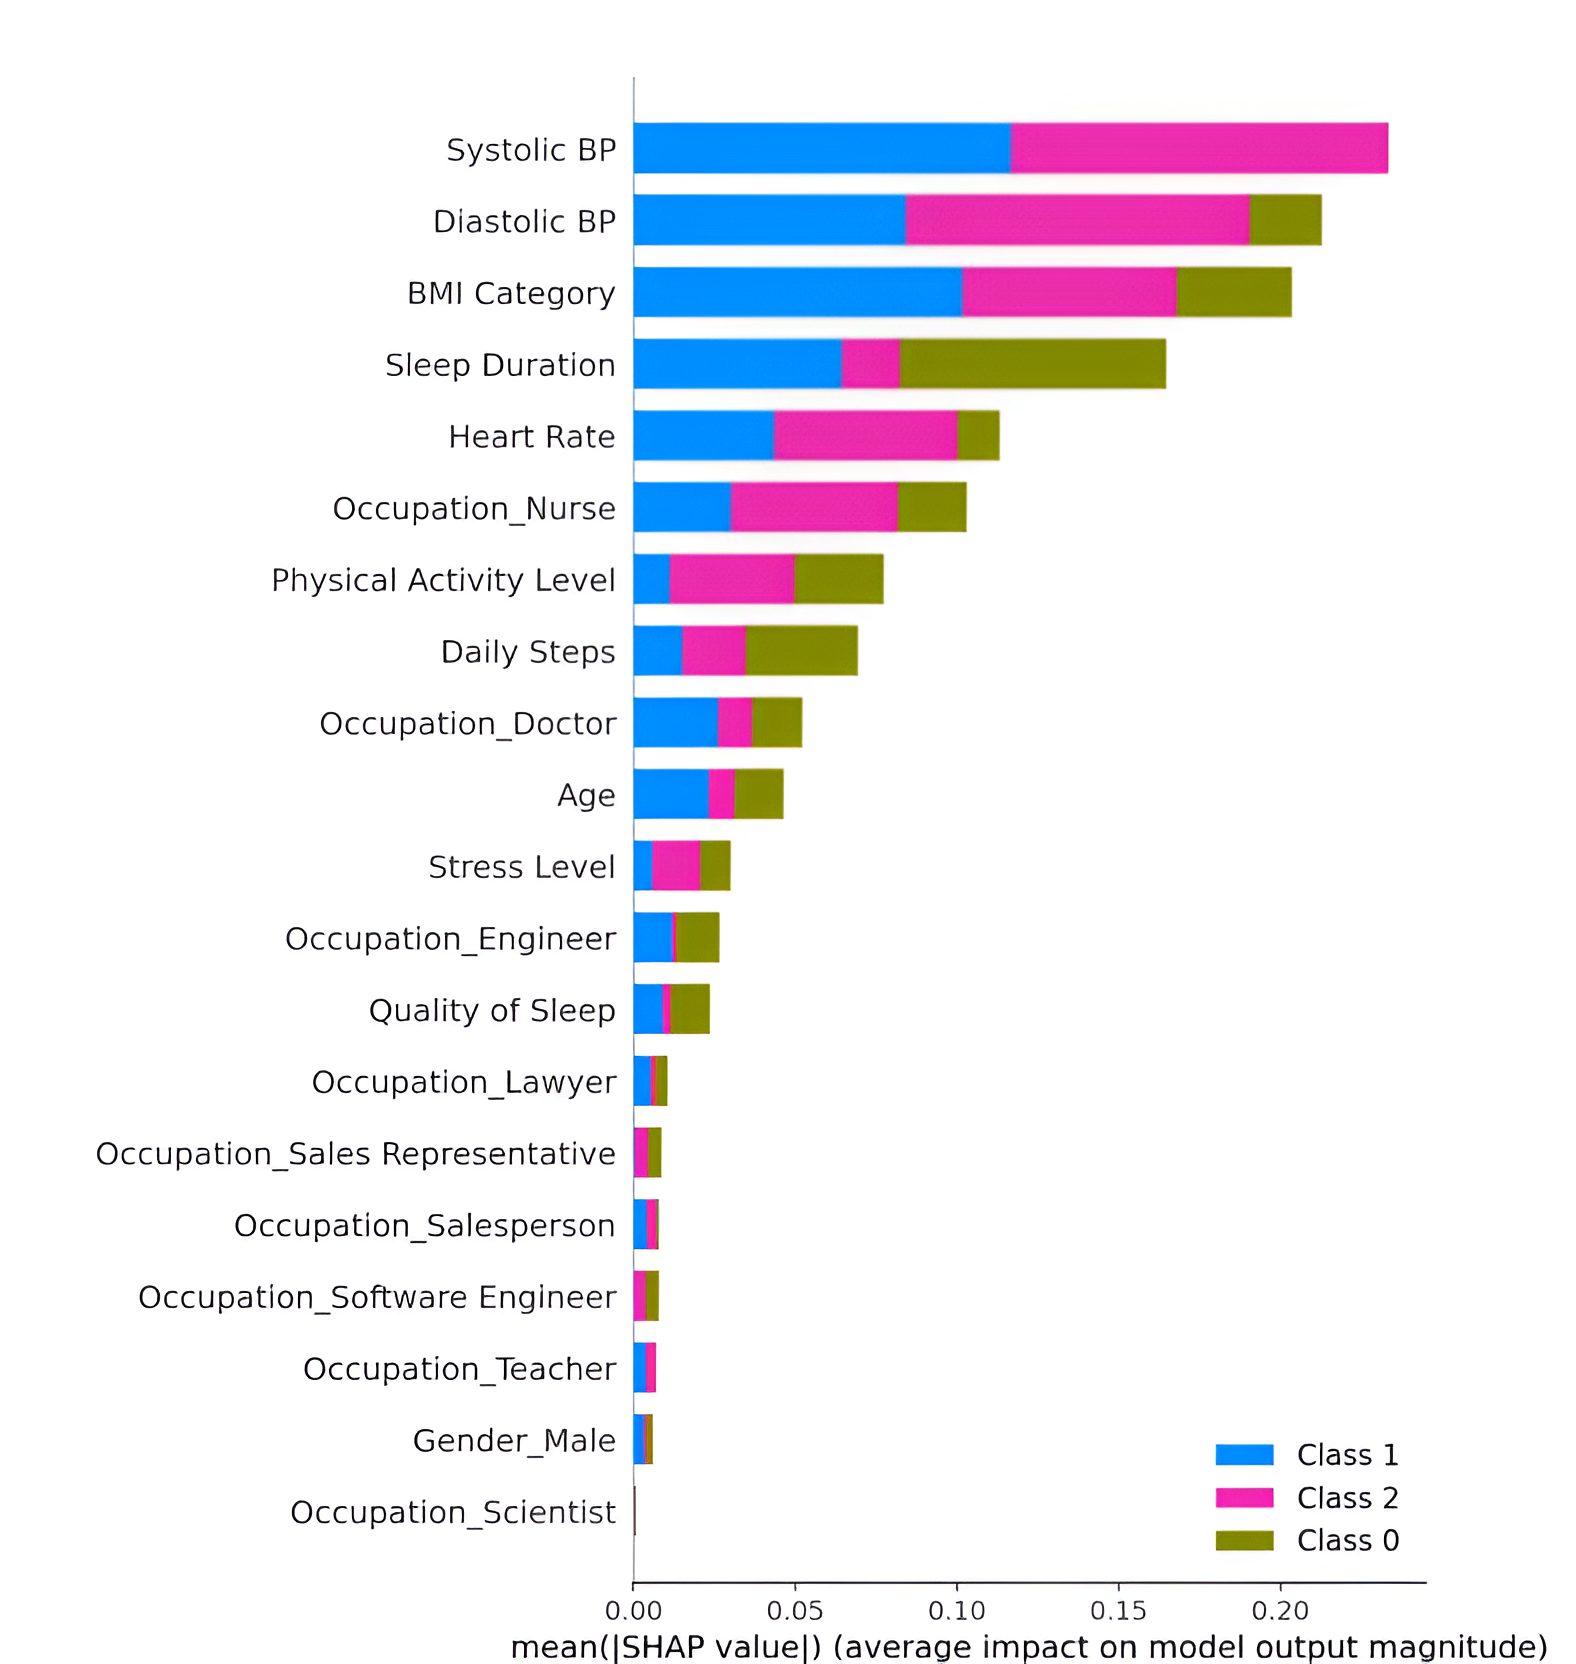
\includegraphics[width=0.9\linewidth]{img/shapApp.png}
    \caption{Gráfico SHAP que representa la importancia de cada variable en la predicción global.}
    \label{fig:shap-global}
\end{figure}

\begin{figure}[H]
    \centering
    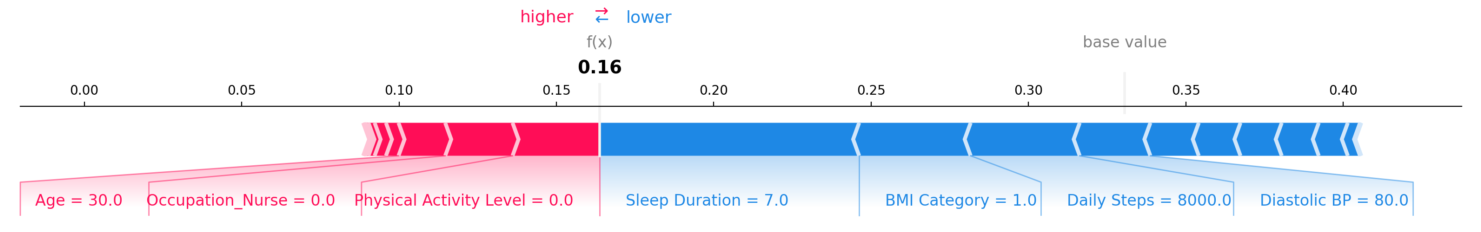
\includegraphics[width=0.8\linewidth]{img/explic_individual.png}
    \caption{Explicación individualizada mediante SHAP para un caso concreto.}
    \label{fig:shap-individual}
\end{figure}

\begin{figure}[H]
    \centering
    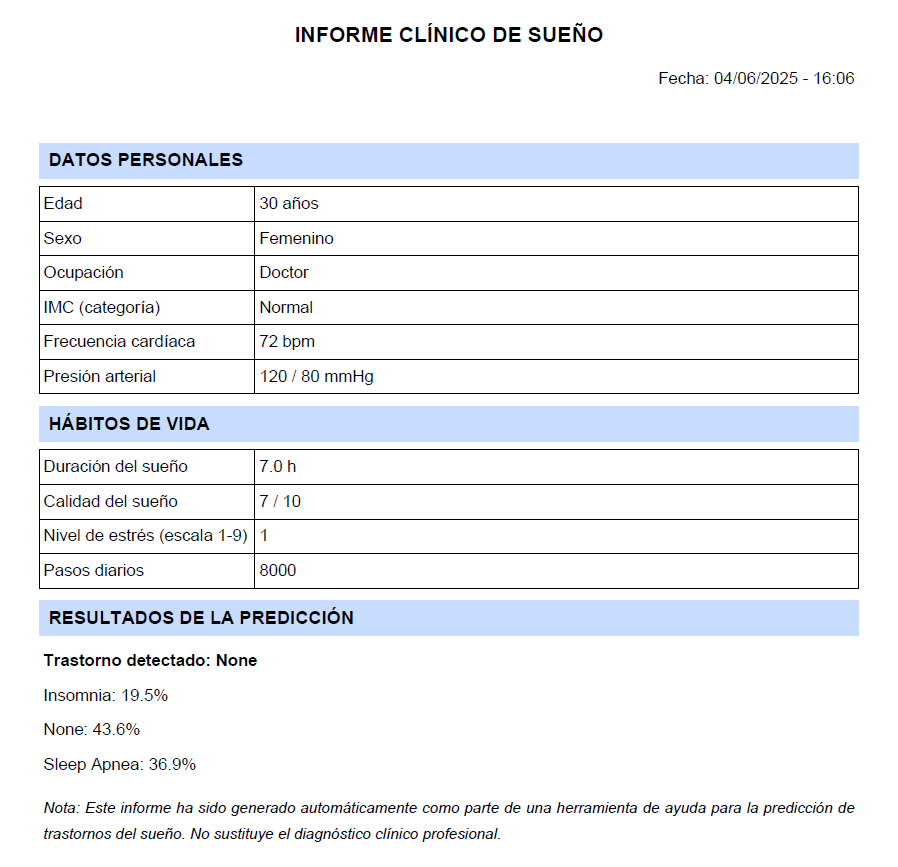
\includegraphics[width=0.9\linewidth]{img/pdfApp.png}
    \caption{Informe clínico en PDF descargado de la aplicación.}
    \label{fig:pdf-app}
\end{figure}

En conjunto, este anexo demuestra que el sistema cumple los requisitos funcionales previstos y ofrece una experiencia de usuario intuitiva, estructurada y coherente con los casos de uso definidos.